\chapter{Układ elektroniczny}
\label{cha:Electronics}
Układ elektroniczny na potrzeby projektu został uproszczony do minimum. Składa się z układu zasilającego, zapewniającego napięcie $12V$ oraz prąd $5A$, oraz gotowej płytki sterownika do silników szczotkowych, do której podpięte są 2 silniki. Dodatkowo płytka jest połączona z komputerem za pomocą kabla USB.

\section{Płytka Nrf Dongle Brushed Motor Controller}

\begin{figure}[h!] 
\centering 
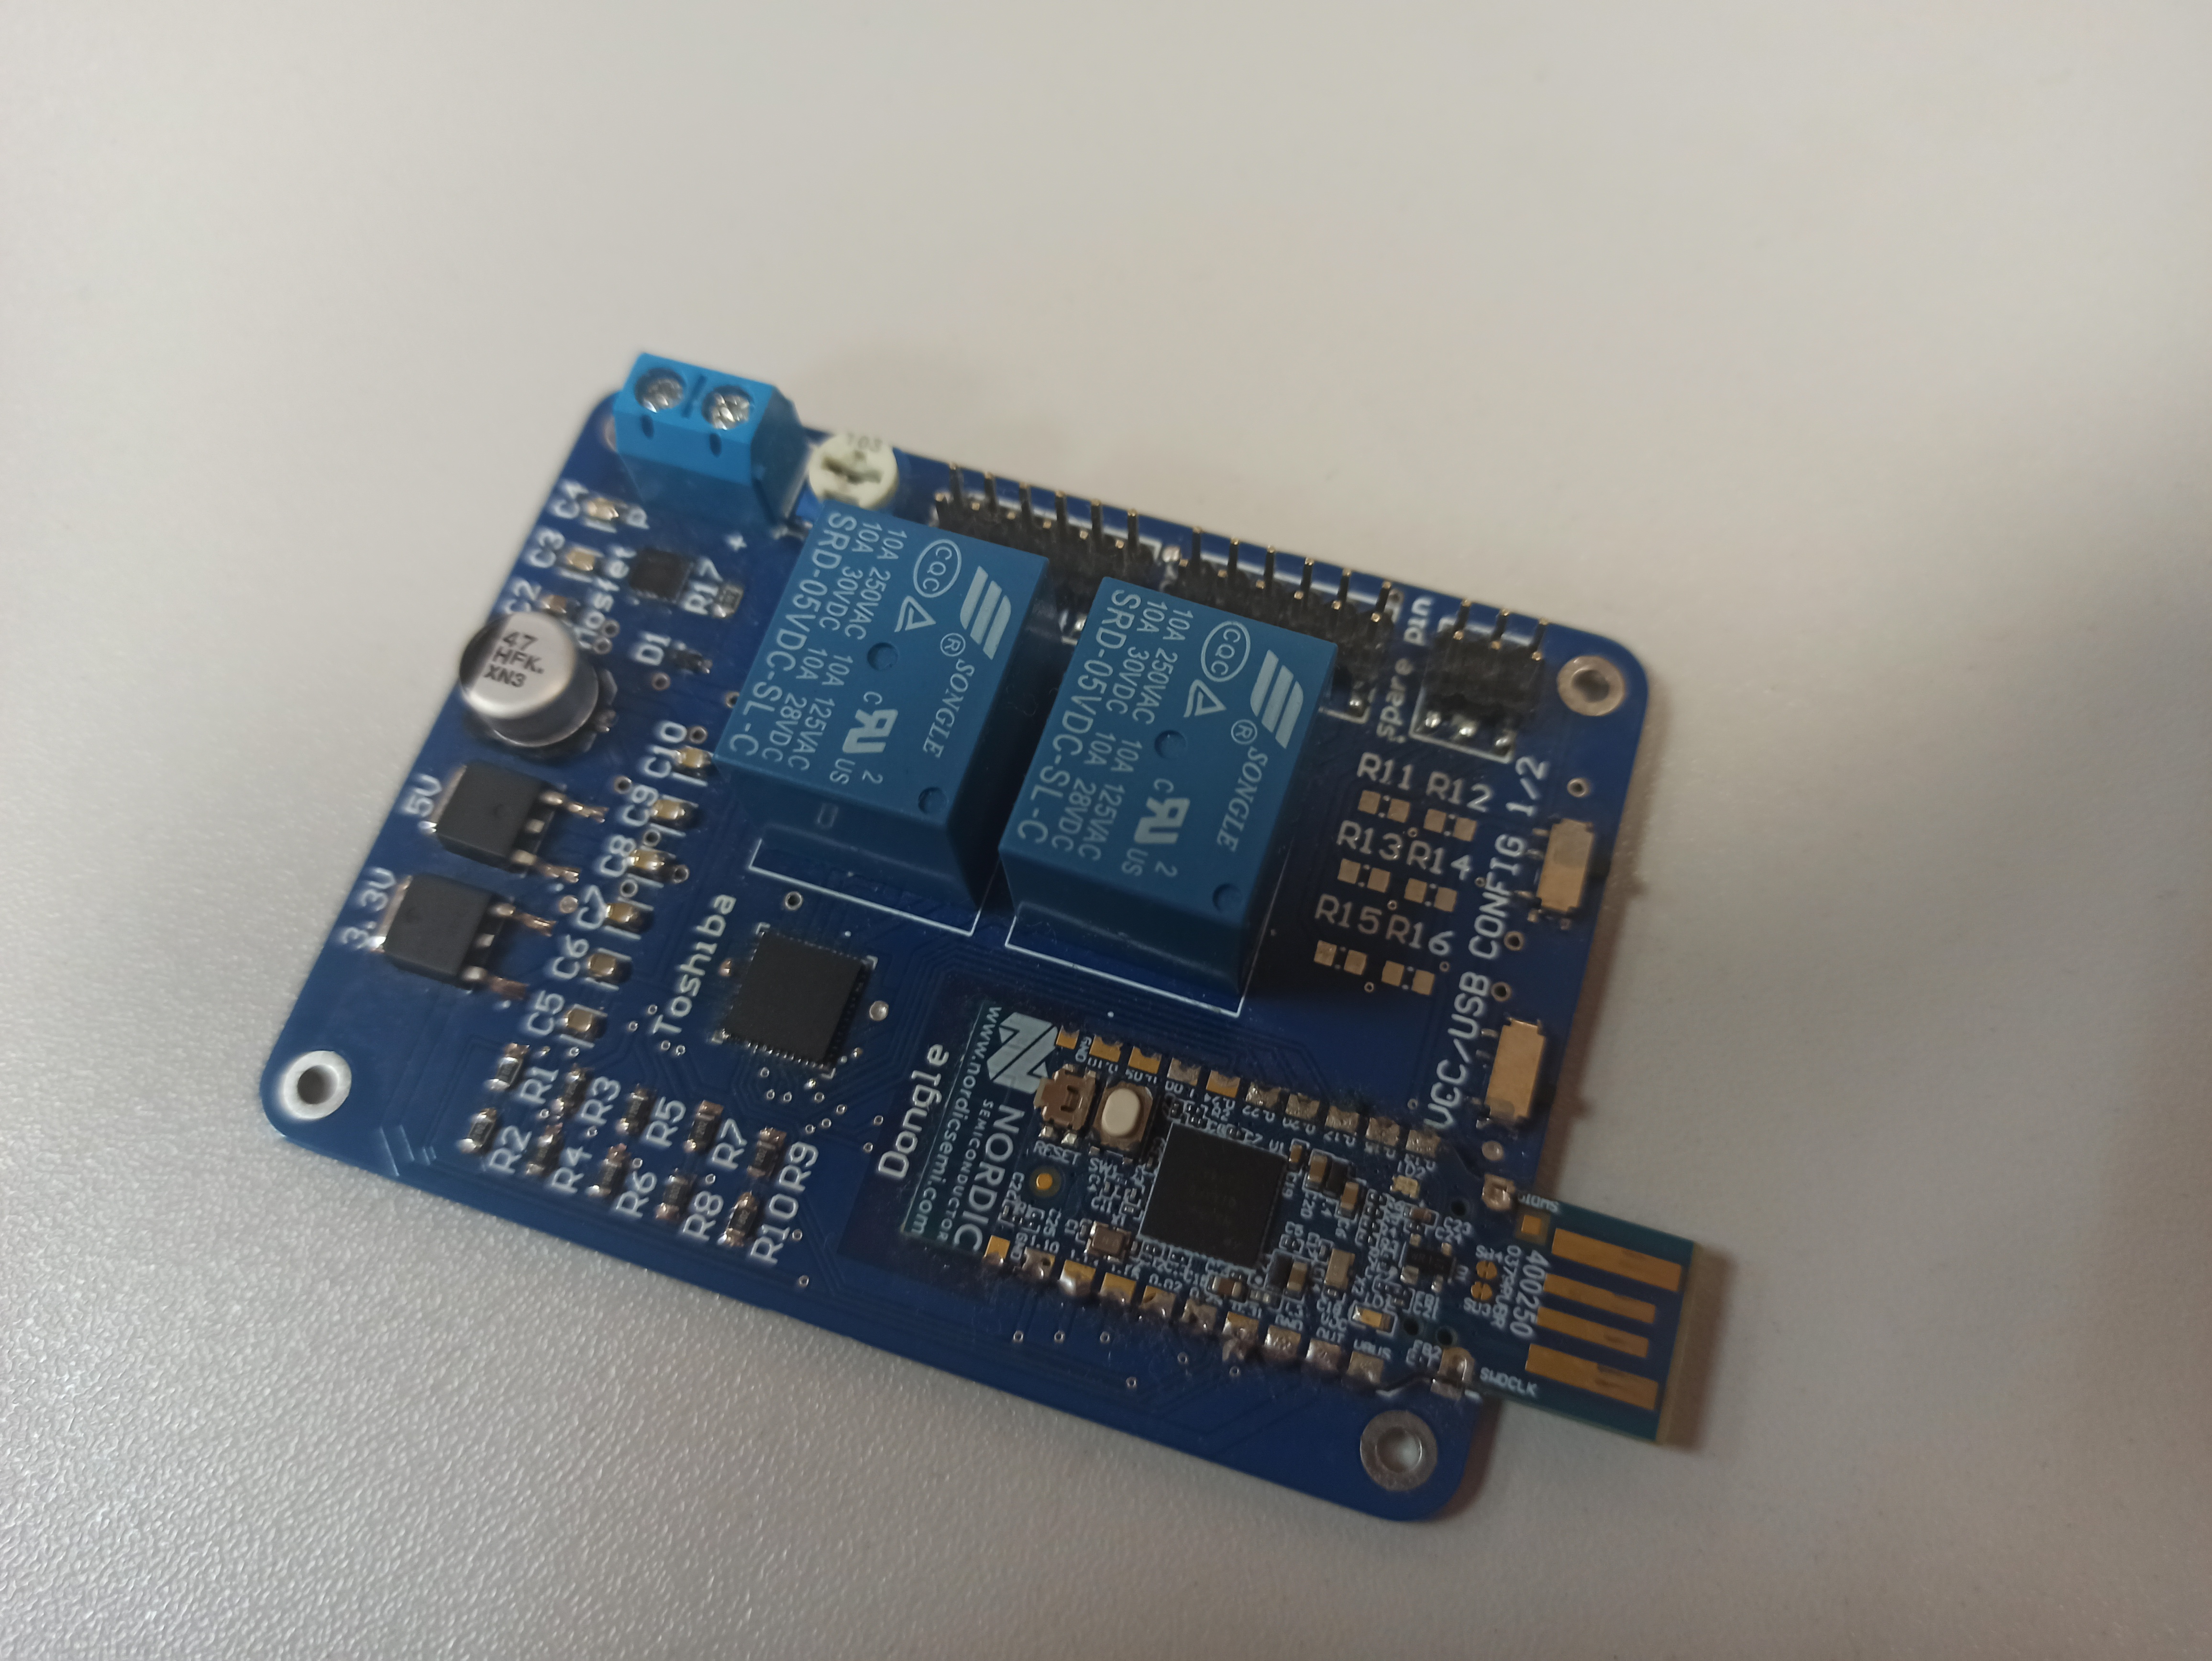
\includegraphics[width=0.8\textwidth]{img/PcbPhoto.jpg}
\caption{Zdjęcie sterownika do silników. Źródło: \cite{nrf_mc_hw}}
\label{img:full_pcb}
\end{figure}

Płytka Nrf Dongle Brushed Motor Controller to układ (przedstawiony na rys. \ref{img:full_pcb}) typu development kit/evaluation board wykonany w kole naukowym "Integra". Układ przede wszystkim składa się z nRF52840 Dongle - płytki prototypowej od firmy Nordic Semiconductors. Procesor nRF52840  kontroluje układ scalony Toshiba TB67H420FTG, który jest dwukanałowym sterownikiem do silników szczotkowych prądu stałego. Na płytce dodatkowo znajdują się 2 układy LDO, które zmniejszają napięcie zasilania z $12V$ do kolejno $5V$ oraz $3.3V$. Linia zasilająca $3.3V$ używana jest do zasilenia mikrokontrolera nRF52840, który jest zasilany napięciem $1.7V$ - $5.5V$. Linia zasilająca $5V$ jest natomiast używana do zasilenia enkodera, który w przypadku silników Pololu 2828 może być zasilany dowolnym napięciem z zakresu $3.5V$ do $20V$. Dodatkowo linie zasilające wyprowadzone są na piny zewnętrzne, aby można było zasilić potencjalne peryferia. Na płytce znajduje się także przeprowadzenie wolnych pinów GPIO (\textbf{General-purpose input/output}, Piny typu Wejście-wyjście ogólnego przeznaczenia) z procesora, oraz przede wszystkim dwa komplety pinów obsługujących silniki z odpowiadającymi im enkoderami. Opisy pinów znajdują się na rewersie płytki.\cite{nrf_mc_hw}



\subsection{nRF52840 Dongle}
\textbf{nRF52840 Dongle} (zdj. \ref{img:full_pcb}) to płytka prototypowa z mikrokontrolerem nRF52840 na pokładzie. Jest programowalna po USB, wspiera większość współczesnych protokołów IoT, jak Bluetooth 5.4, Thread czy Zigbee. Posiada też programowalne 2 diody, przycisk, jak i 15 wyprowadzeń typu GPIO. \cite{nrf_dongle}

\begin{figure}[h!] 
\centering 
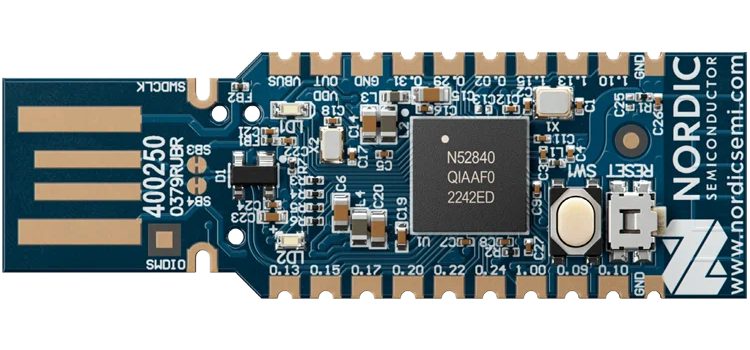
\includegraphics[width=0.4\textwidth]{img/nRF52840_Dongle.png}
\caption{nRF52840 Dongle. Źródło: \cite{nrf_dongle}}
\label{img:full_pcb}
\end{figure}

Na potrzeby sterownika do silników użyte zostało 12 pinów GPIO, 3 zostały przeprowadzone na zewnętrzne piny. Wyprowadzenia pinów układu nRF52840 Dongle:
\begin{itemize}
    \item 0.13 - PWM kanału B, połączone z układem Toshiby, odpowiada za kontrolę prędkości silnika B.
    \item 0.15 - PWM kanału A, jak wyżej.
    \item 0.17 - LO1, kod błędu zwracany przez układ Toshiby
    \item 0.20 - LO2, kod błędu zwracany przez układ Toshiby
    \item 0.22 - IN1 kanału A, pierwszy pin sterujący, odpowiadający za ustawienie kierunku ruchu silnika
    \item 0.24 - IN2 kanału A, drugi pin sterujący, jak wyżej.
    \item 1.00 - IN1 kanału B, jak wyżej.
    \item 0.09 - IN2 kanału B, jak wyżej.
    \item 0.10 - Enkoder 2 kanału B - pin odpowiadający za sprzężenie zwrotne od enkodera.
    \item 0.31 - P3, pin wolny przeprowadzony na zewnętrzny header.
    \item 0.29 - P1, jak wyżej.
    \item 0.02 - P2, jak wyżej.
    \item 1.15 - Enkoder 1 kanału A - pin odpowiadający za sprzężenie zwrotne od enkodera.
    \item 1.13 - Enkoder 2 kanału A - jak wyżej.
    \item 1.10 - Enkoder 1 kanału B - jak wyżej.
\end{itemize} \cite{nrf_mc_hw}

Znajomość wyżej opisywanych wyprowadzeń będzie przydatna w rozdziale \ref{cha:Software}, przy opracowywaniu oprogramowania odpowiedzialnego za kontrolę silnika.

\subsection{Toshiba TB67H420FTG Motor Controller}

TB67H420FTG to chip sterownika silników szczotkowych prądu stałego. Wewnętrzny mostek H można skonfigurować jako podwójny mostek dla jednego silnika, lub dwa pojedyncze mostki sterujące niezależnie dwoma osobnymi silnikami. Na potrzeby tego projektu opcja ta jest permanentnie ustawiona na dwa niezależne silniki za pomocą fizycznego przycisku na płytce, który zwiera odpowiedni pin chipu do masy. \cite{Toshiba_docs}

Jednakże najważniejsze piny z punktu widzenia tej pracy to piny mostka H, czyli IN1, IN2 oraz PWM, odpowiednio A i B w zależności od kanału. Opisują one zachowanie silnika w zależności od wejścia, jakie podamy na sterownik Toshiby. Zachowanie silnika w zależności od wartości tych 3 pinów przedstawia tabela \ref{table:Toshiba_pins}. W tabeli tej L oznacza stan niski pinu, zwarcie z masą, natomiast H stan wysoki, zwarcie z VCC. Należy także dodać, że jest to uproszczona wersja tabeli znajdującej się w rozdziale 3 dokumentacji \cite{Toshiba_docs}.

\begin{table}[h!]
\centering
\begin{tabular}{c | c c | c }
 PWM & IN1 & IN2 & tryb pracy silnika \\
 \hline
L & L & L & Standby Mode \\
L & - & - & Short Brake \\
H & L & L & Stop \\
H & H & L & Forward Rotation \\
H & L & H & Reverse Rotation \\
H & H & H & Short Brake \\
\end{tabular}
\caption{Uproszczona tabela trybów pracy sterownika TB67H420FTG. Źródło: \cite{Toshiba_docs}}
\label{table:Toshiba_pins}
\end{table}

Z punktu widzenia pisania późniejszego oprogramowania, można założyć, że Standby zachowuje się identycznie jak Stop. Tryby te powodują, że na silnik nie jest podawany prąd. Short Brake natomiast powoduje nagłe hamowanie oraz blokadę silnika. W tym trybie, prąd jest cały czas podawany na wyjście, co powoduje utrzymywanie silnika w miejscu. Najciekawsze natomiast są tryby Rotation, w których, jak sama nazwa wskazuje, silnik obraca się w zadanym kierunku, z prędkością proporcjonalną do wartości wypełnienia PWM.